\documentclass[12pt,pdf,hyperref={unicode}]{beamer}


%\documentclass[10pt]{beamer}

\usetheme[progressbar=frametitle]{metropolis}

\usepackage{booktabs}
\usepackage[scale=2]{ccicons}

\usepackage{pgfplots}
\usepgfplotslibrary{dateplot}

\usepackage{xspace}
\newcommand{\themename}{\textbf{\textsc{metropolis}}\xspace}


%\usepackage{lmodern}

% подключаем кириллицу 
\usepackage[T2A]{fontenc}
\usepackage[utf8]{inputenc}
\usepackage{listings}
%\usepackage{graphicx}
\usepackage{hyperref}

% отключить клавиши навигации
\setbeamertemplate{navigation symbols}{}

% тема оформления
\usetheme{Pittsburgh}

% цветовая схема
\usecolortheme{default}

\definecolor{light-gray}{gray}{0.90}

\title{Семинар №9}   
\subtitle{ФАКИ \the\year}
\author{Бирюков В. А.} 
\date{\today}
% \logo{\includegraphics[height=5mm]{images/logo.png}\vspace{-7pt}}

\begin{document}

\lstset{language=C}

% титульный слайд
\begin{frame}
\titlepage
\end{frame} 

\defverbatim[colored]\makeset{
\begin{lstlisting}[language=C++,basicstyle=\ttfamily,keywordstyle=\color{blue}]
void make_set(int X) {
  parent[X] = X;
}
\end{lstlisting}
}

\lstset{
  language=C,                % choose the language of the code
  keywordstyle=\color{blue},
  numbers=none,                   % where to put the line-numbers
  stepnumber=1,                   % the step between two line-numbers.        
  numbersep=5pt,                  % how far the line-numbers are from the code
  backgroundcolor=\color{light-gray},  % choose the background color. You must add \usepackage{color}
  showspaces=false,               % show spaces adding particular underscores
  showstringspaces=false,         % underline spaces within strings
  showtabs=false,                 % show tabs within strings adding particular underscores
  tabsize=2,                      % sets default tabsize to 2 spaces
  captionpos=b,                   % sets the caption-position to bottom
  breaklines=true,                % sets automatic line breaking
  breakatwhitespace=true,         % sets if automatic breaks should only happen at whitespace
}

\begin{frame}[fragile]
\frametitle{Память под локальные переменные} 
\begin{center}
\includegraphics[width=\linewidth]{images/v_stack1.png}
\end{center}
\end{frame}

\begin{frame}[fragile]
\frametitle{Память под локальные переменные} 
\begin{center}
\includegraphics[width=\linewidth]{images/v_stack2.png}
\end{center}
\end{frame}

\begin{frame}[fragile]
\frametitle{Память под локальные переменные} 
\begin{center}
\includegraphics[width=\linewidth]{images/v_stack3.png}
\end{center}
\end{frame}

\begin{frame}[fragile]
\frametitle{Память под локальные переменные} 
\begin{center}
\includegraphics[width=\linewidth]{images/v_stack4.png}
\end{center}
\end{frame}

\begin{frame}[fragile]
\frametitle{Память под локальные переменные} 
\begin{center}
\includegraphics[width=\linewidth]{images/v_stack5.png}
\end{center}
\end{frame}

\begin{frame}[fragile]
\frametitle{Память под локальные переменные} 
\begin{center}
\includegraphics[width=\linewidth]{images/v_stack6.png}
\end{center}
\end{frame}

\begin{frame}[fragile]
\frametitle{Сегмент памяти: Стек вызовов} 
\begin{center}
\includegraphics[width=\linewidth]{images/v_stack7.png}
\end{center}
\end{frame}



\begin{frame}[fragile]
\frametitle{Управление памятью} 
\framesubtitle{Сегменты памяти процесса}
\begin{center}
\includegraphics[width=0.9\linewidth]{images/process_memory_organization.png}
\end{center}
\end{frame}




\begin{frame}[fragile]
\frametitle{Сегменты памяти: Стек вызовов (Call stack)} 
\begin{itemize}
\item Стек представляет собой обычный алгоритмический стек, применённый для управления памяти
\item В нём хранятся локальные переменные
\item Имеет фиксированный размер, определяется операционной системой, на порядок меньше чем Куча
\item Быстрее, чем Куча
\end{itemize}
\end{frame}

\begin{frame}[fragile]
\frametitle{Сегменты памяти: Куча (Heap)} 
\begin{itemize}
\item Куча представляет собой обычную алгоритмическую кучу, применённую для управления памяти
\item В ней можно динамически выделять память
\item Размер, обычно, ограничен только доступными ресурсами
\item Медленней, чем Стек
\end{itemize}
\end{frame}


\begin{frame}[fragile]
\frametitle{Сегменты памяти: Текст (Text)} 
\includegraphics[width=0.99\linewidth]{images/c_to_byte.jpg}
\end{frame}


\section{Алгоритмы}



\begin{frame}[fragile]
\frametitle{Алгоритм} 
\begin{itemize}
\item Алгоритм -- это формально описанная вычислительная процедура, получающая исходные данные, и выдающая результат
вычислений на выход \\
(Кормен и др. "Алгоритмы: построение и анализ")
\end{itemize}
\end{frame}


\begin{frame}[fragile]
\frametitle{Сортировки} 
\begin{itemize}
\item Простейшие:
\begin{itemize}
\item Сортировка вставками \\
\item Сортировка выбором \\
\item Сортировка пузырьком \\
\end{itemize}
\item Чуть сложнее:
\begin{itemize}
\item Сортировка слиянием \\
\item Быстрая сортировка \\
\item Цифровая сортировка \\
\end{itemize}
\end{itemize}
\end{frame}


\section{Анализ алгоритмов}

\begin{frame}[fragile]
\frametitle{Анализ алгоритмов} 
\begin{itemize}
\item Обычно изучают зависимость времени работы от размера входа \\
\item Размер входа -- зависит от конкретной задачи \\
\item Для сортировки, размер входа -- это количество элементов, которые нужно отсортировать \\
\item Время работы -- число элементарных шагов, которые выполняет алгоритм
\end{itemize}
\end{frame}

\begin{frame}[fragile]
\frametitle{Пример анализа} 
\framesubtitle{Сортировка пузырьком}
\begin{lstlisting}[language=C++,basicstyle=\ttfamily,keywordstyle=\color{blue}]
for (int j = 0; j < length-1; j++)
    for (int i = 0; i < length-1; i++)
         if (a[i] > a[i+1])
             swap(a[i], a[i+1]);
\end{lstlisting}
\begin{itemize}
\item Число операций, требуемых на один проход: $a * n$\\
\item Число проходов: $n$\\
\item Значит, время работы $\sim n^2$\\
\end{itemize}

\end{frame}


\section{Принцип "разделяй и влавствуй". Сортировка слиянием и быстрая сортировка}

\begin{frame}[fragile]
\frametitle{Принцип "разделяй и влавствуй"} 
\begin{itemize}
\item Задача разбивается на несколько подзадач меньшего размера \\
\item Эти задачи решаются (обычно с помощью рекурсивного вызова) \\
\item Решения этих задач комбинируются и получается решение исходной задачи \\
\end{itemize}
\end{frame}

\begin{frame}[fragile]
\frametitle{Сортировка слиянием} 
\begin{center}
\includegraphics[width=0.9\linewidth]{images/mergeSort.png}
\end{center}
\end{frame}


\begin{frame}[fragile]
\frametitle{Сортировка слиянием} 
\begin{center}
\includegraphics[width=0.9\linewidth]{images/mergeSort_pseudo.png}
\end{center}
\end{frame}



\begin{frame}[fragile]
\frametitle{Принцип "разделяй и влавствуй" для сортировки} 
\frametitle{Быстрая cортировка (quicksort)} 
\begin{itemize}
\item Выбираем в массиве некоторый элемент, который будем называть опорным \\
\item Переставляем элементы массива таким образом, чтобы все элементы со значением меньшим или равным опорному элементу, оказались слева от него, а все элементы, превышающие по значению опорный — справа от него \\
\item Рекурсивно сортируем подмассивы, лежащие слева и справа от опорного элемента\\
\end{itemize}
\end{frame}

\begin{frame}[fragile]
\frametitle{Быстрая cортировка (quicksort)} 
\begin{center}
\includegraphics[width=0.9\linewidth]{images/qs1.png}
\end{center}
\end{frame}

\begin{frame}[fragile]
\frametitle{Быстрая cортировка (quicksort)} 
\begin{center}
\includegraphics[width=0.9\linewidth]{images/qs2.png}
\end{center}
\end{frame}


\section{Время работы сортировок}

\begin{frame}[fragile]
\frametitle{Время работы сортировок} 
\begin{itemize}
\item Время работы сортировки пузырьком, выбором и вставками $\sim n^2$ \\
\item Время работы сортировки слиянием и быстрой сортировки в среднем $\sim n log(n)$ \\
\end{itemize}
\end{frame}

\begin{frame}[fragile]
\frametitle{Время работы сортировок} 
\begin{itemize}
\item Пусть мы хотим отсортировать массив из 1 млн. чисел
\item Сортировка пузырьком написана аккуратно и требует $2n^2$ операций и выполняется на суперкомпьютере(x100)
\item Сортировка слиянием написана неэффективно и требует $50 n log(n)$ операций и выполняется на пк(x1)
\item Сортировка пузырьком выполнится за 5.5 часов \\
\item Сортировка слиянием выполнится за 17 минут \\
\end{itemize}
\end{frame}


%E9C6AF
%C6E9AF


\section{Стандартная сортировка qsort()}


\begin{frame}[fragile]
\frametitle{Стандартная сортировка qsort()} 
\begin{lstlisting}[language=C++,basicstyle=\ttfamily,keywordstyle=\color{blue}]
#include <stdlib.h>
int values[] = { 88, 56, 100, 2, 25 };

int cmp(const void * a, const void * b)
{
   return ( *(int*)a - *(int*)b );
}
...
qsort(values, 5, sizeof(int), cmp);

\end{lstlisting}
\end{frame}



\end{document}
